In order to have the upper bound of the  adaptivity of a program $c$, we design a program analysis framework {\THESYSTEM}. It can be divided as two steps: 1) to construct a weighted dependency graph based on $c$. 2) to find a path in this graph, which is used to estimate an upper bound on the adaptivity of $c$.
\begin{figure}
  \centering    
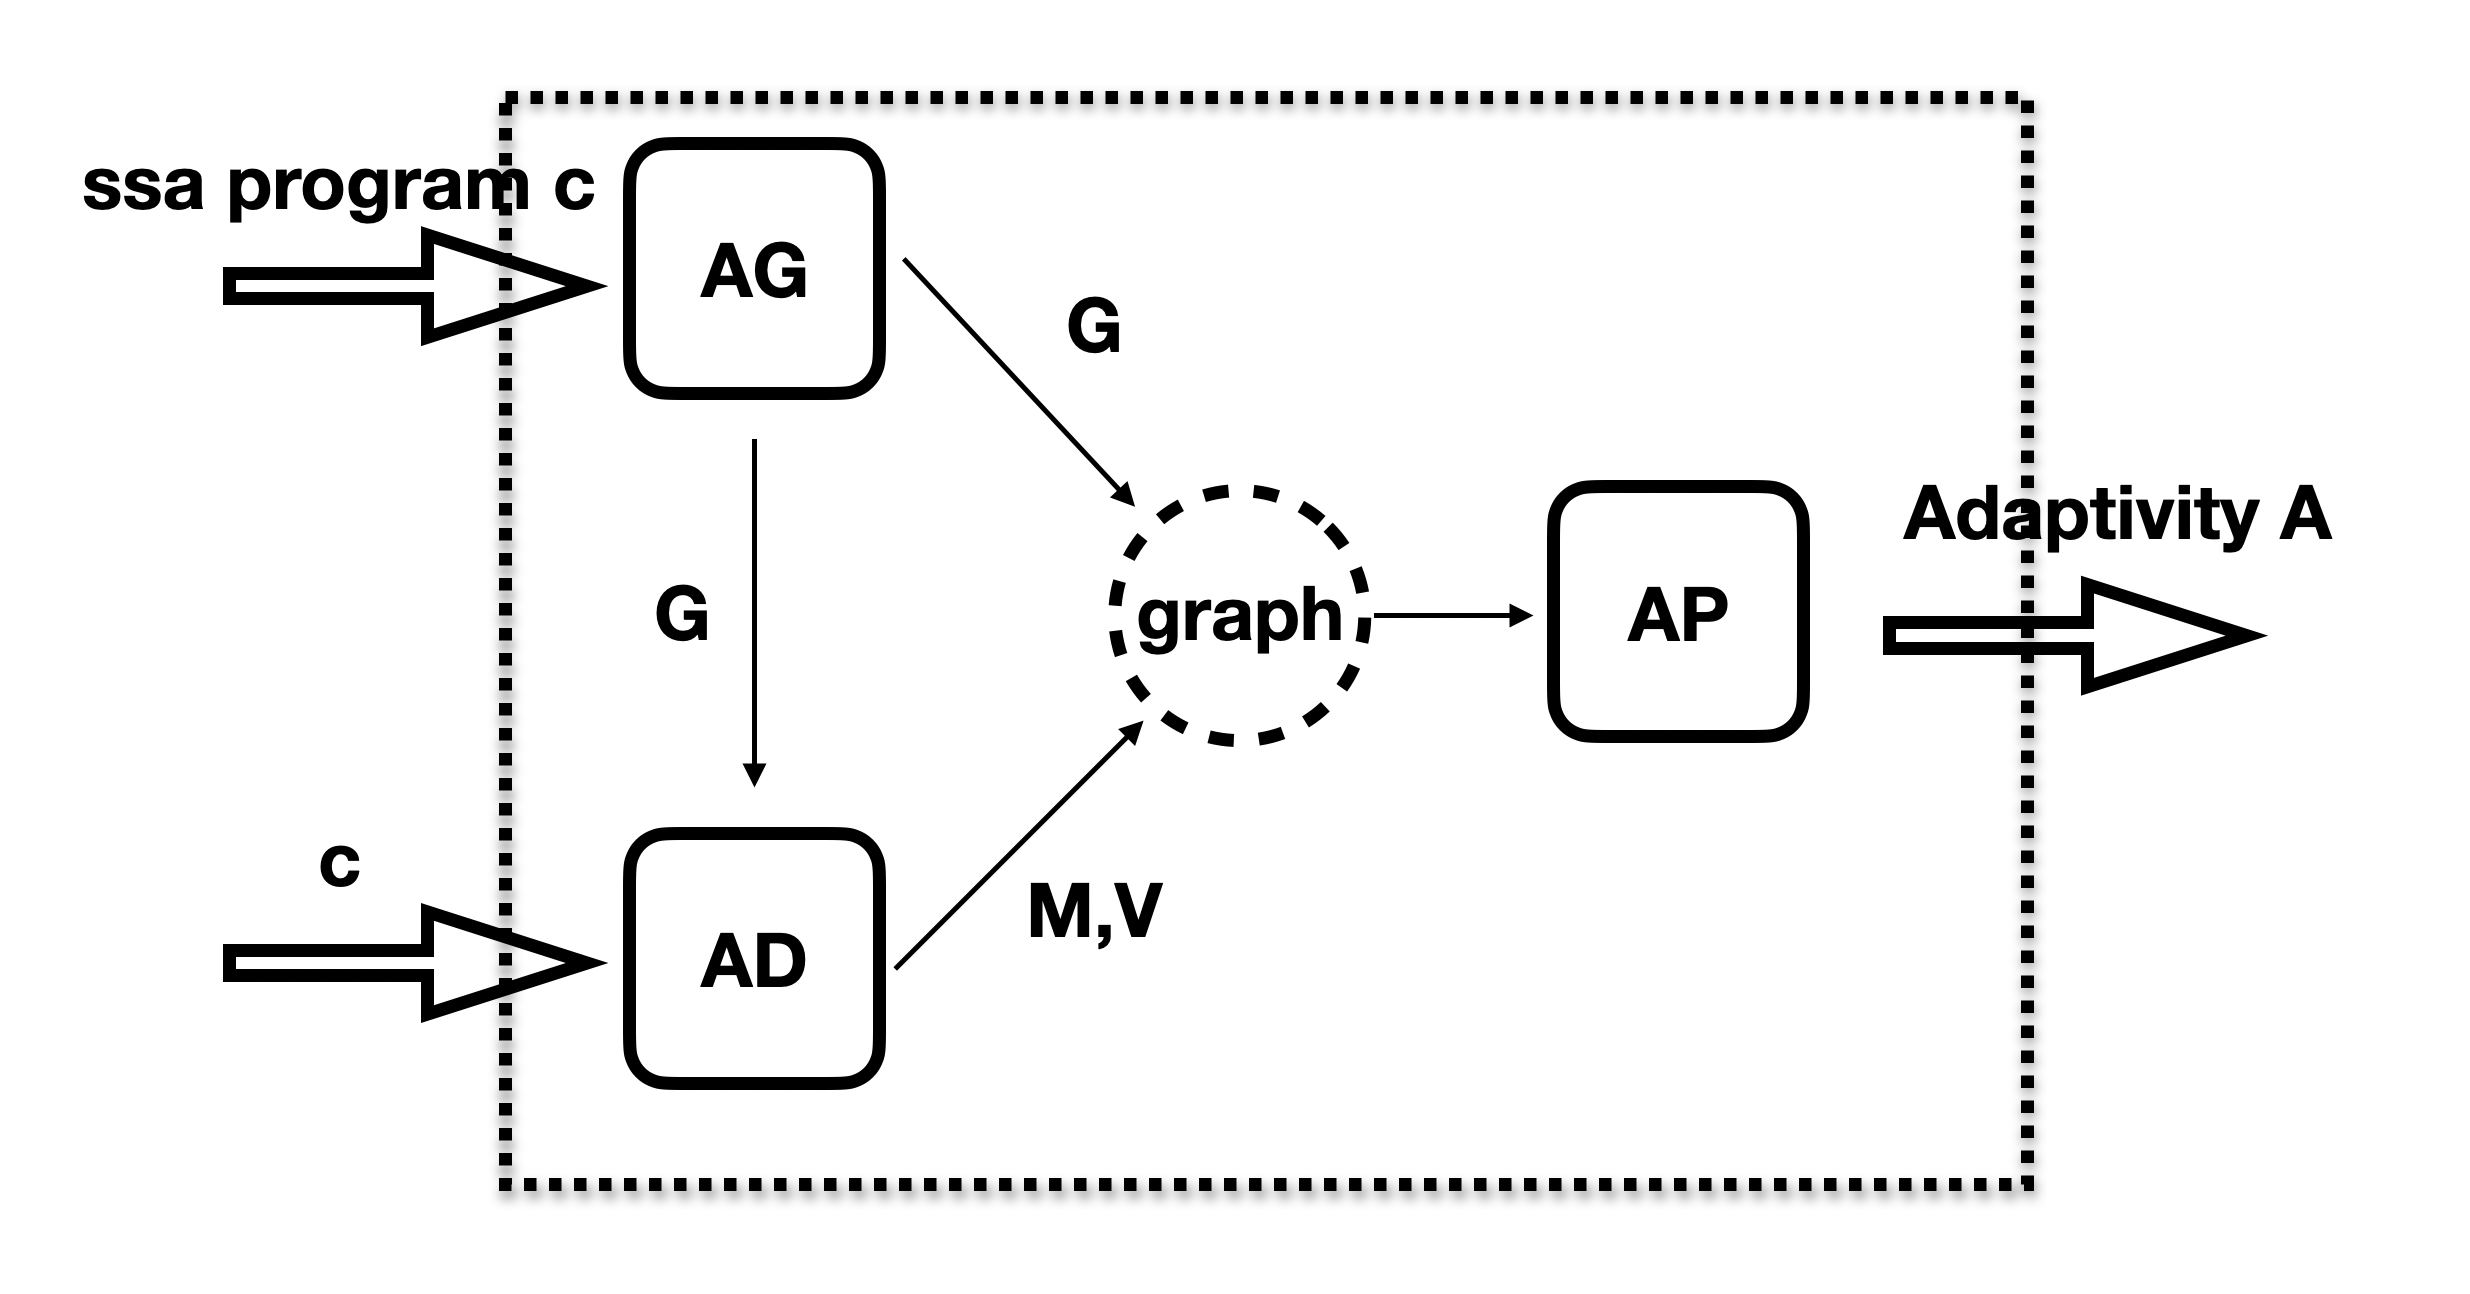
\includegraphics[width=1.0\columnwidth]{adapfun.png}
  \vspace{-0.3cm}
  \caption{The overview of {\THESYSTEM}}
  \label{fig:adaptfun}
  \vspace{-0.5cm}
\end{figure}
\subsubsection{Graph Estimation}
%
%
According to the dependency graph we use in adaptivity definition, we want to build a similar graph to {over-}approximate the
% execution-based dependency graph (in Definition~\ref{def:trace_graph})
Execution-Based Dependency Graph (in Definition~\ref{def:trace_graph}). The construction considers the vertices, edges, and the weight of every node, as well as some annotations which marks the query usage. The overall picture of this step is organized as follows.
% through Section~\ref{sec:alg_vertexgen}, Section~\ref{sec:alg_weightedgegen} and~\ref{sec:alg_graphgen}:


\begin{enumerate}
\item  Vertices are the assigned variables with unique labels, which is extracted directly from the program, see Section~\ref{sec:alg_vertexgen}
without extra static analysis technique.git 
\item Query annotations are also decided directly from the program, when there is a query request, the associated variables which are the results of the query requests are marked in the form of a flag, $0$ means no query, $1$ represents query related. See Section~\ref{sec:alg_vertexgen}.
\item Every vertice has a weight, which tells the maximal times this vertices can be visited in realistic execution. This weight is estimated by a reachability bound analysis on each vertice, See Section~\ref{sec:alg_weightgen}.
\item The edges between vertices considers both control flow and data flow, See
Section~\ref{sec:alg_edgegen}
\item  Finally, with all the ingredients ready, we construct the final approximated program-based dependency graph in Section~\ref{sec:alg_graphgen}
\end{enumerate}

% the algorithm  without extra static analysis technique.
% \\
Overall, this program-based graph has a similar topology structure as 
% the one
% of 
the Execution-Based Dependency Graph. It has the same
vertices and query annotations, but approximated edges and weights. We call the graph generated by static analysis techniques, static analysis dependency graph. 

\subsubsection{Adaptivity Computation}

Likewise the adaptivity is defined as a finite walk in the execution based dependency graph, 
our static estimation on this adaptivity also relies on finding a path in the static analysis dependency graph.
The construction of the stastic analysis dependency graph is of great value of showing some useful properties of the target program, such as dependency between variables, 
the execution upper bound of a certian command, while the key novelty is our path searching algorithm, which connects all the information we need in the static analysis dependency graph and provides us a sound over-estimation of adaptivity! 
In order to get a sound but precise upper bound, 
we will discuss some challenges in finding the 'appropriate' path in the graph, and how our algorithm responds to these challenge. We present the path searching algorithm in Section~\ref{sec:static-adapt}.